% Created 2023-09-15 Fri 19:54
% Intended LaTeX compiler: pdflatex
\documentclass[11pt]{article}
\usepackage[utf8]{inputenc}
\usepackage[T1]{fontenc}
\usepackage{graphicx}
\usepackage{longtable}
\usepackage{wrapfig}
\usepackage{rotating}
\usepackage[normalem]{ulem}
\usepackage{amsmath}
\usepackage{amssymb}
\usepackage{capt-of}
\usepackage{hyperref}
\author{Tim Hawes}
\date{\today}
\title{Naurrnen}
\hypersetup{
 pdfauthor={Tim Hawes},
 pdftitle={Naurrnen},
 pdfkeywords={},
 pdfsubject={},
 pdfcreator={Emacs 28.2 (Org mode 9.6.1)}, 
 pdflang={English}}
\begin{document}

\maketitle
\tableofcontents

\section{Secret Origins}
\label{sec:orgf664b94}
\subsection{Introduction}
\label{sec:org326a72f}
This file contains spoilers for the world of Naurrnen. What is the difference between science and magic? The difference, I believe, is far more subtle and blurry than one in our modern age might be willing to admit. Science is being able to explain phenomenon as a form of a satisfactory answer as to the what and why of what happens, and formulating that explanation as a consistent repeatable system. Magic is simply the exceptions to the known rules of science, that have not yet received an explanation of how the phenomenon fits the larger explainable scientific world. Beyond that, magic and science are hardly distinguishable. Men and women's conquest to learn more, I believe, is an infinite journey that never arrives to its destination. Given that, there will ever be both the phenomenal and noumenal.

\subsection{Gravity Mining}
\label{sec:org689587c}
Gravity mining is the process of creating entirely new substances through the use of extremely strong gravitational pull, from the likes of a neutron star or black hole. The easiest manner to describe this process in the real world, is essentially, two particles are bound through quantum mechanics, and once bound, one particle is isolated in a gravity-free container, at absolute zero, and the other is flung into a neutron star or black hole. At a certain point, the linked particle is unlinked, and is something entirely different. What substance you ended up with depended entirely on the starting mass, the gravitational pull of the other particle, the link strength of the two particles, and at which stage the unlinking process begun. The linking and unlinking processes became known as ``quantum linking''. Because the actual matter being used matters very little, and the abundance of matter to use for the process, and even the ability to recycle the created substances, it is possible to mass produce several entirely new substances. Two of the most common substances produced are a super fuel for space travel, and metal that can withstand speed of light travel.

\subsection{Planetary Commerce}
\label{sec:org3c8ffb5}
Given the distance between solar systems, it became expedient to send space stations to un-inhabitable systems for the purpose of refueling, and maintenance of cargo ships. Initially, these stations were sent to orbit various planets in these systems. Profitable enterprises would build these stations, and sell fuel, maintenance and entertainment. As demand grew for waypoints with lots of trade traffic, these stations would be expanded. Often, in many higher traffic stations, they were expanded to the size of small moons, and then the size of planets that would be relocated from a planetary orbit to a solar orbit. Thus the beginning of synthetic planetary systems. The progression was something like space station to synthetic moon, to synthetic planet. When inter-galactic trade routes extended beyond what was convenient, a less expensive alternative was formed for creating way points along the trade routes. This gave way to terraforming planets to make them habitable. It was far more economic to start a populace on a terraformed planet using incubation pods. Where literally hundreds of thousands of fertilized human and alien embryos could be nurtured and grown. Artificial intelligence had made it possible to nurture embryos that were ready to become infants in the outside world.

I want to make some things clear. The AI that cared for the embryos were not sentient, and only covered the biological care of the embryos. Prior to embryo hatching, tutors and educators would arrive and prepare for instructing the new life in how to build its own unique culture and participate in interstellar trade.

The alien races are what the high fantasy reader might identify as men, dwarves, elves, and orcs. There are no explicitly evil races, just very different species each with their own unique gifts, talents, and culture over time.

\subsubsection{Naurrnen (Syscon 37221)}
\label{sec:org66aca0a}
Syscon 37221 was one such planet. When the trade route dried up, the populace was relocated and the planet abandoned. Or so it was thought. Records indicate that there were numerous pods abandoned to the AI to raise without any monitoring at all. It looks like a bureaucratic cover-up in order to avoid costly relocation of equipment. When the coverup was discovered, a recovery mission was sent in order to re-assume the hatched embryos into society, and possibly recover any equipment that might be salvageable. The system in which the planet was part of was no more. Swallowed up by a neighboring worm hole for sure, it would seem. If the planet still existed, it was unreachable, now.

\subsection{Fantasy}
\label{sec:org50779a3}
Having started this world with many potential ``sci-fi'' underpinnings, it is also essential to fill this world with fantasy. Let the imagination run without the confines of understood reality. With enough mystery, inhabitants of this world will tell their stories and their own unique interpretation of the world around them. They must have the freedom to do this, for this is what makes a make-believe world welcoming.

\subsection{Ideas}
\label{sec:org95679af}
\begin{enumerate}
\item Active satellites still orbiting and still self correcting orbital path, that interact with the planet, and ``magical artifacts'' i.e. staff that calls fire (lasers?) or nanite robots that repair tissue
\item EMP devices that are interpreted to be ``anti-magical''
\item solar energy as a possible source of renewable energy
\item terraformed planet
\end{enumerate}
\section{World}
\label{sec:orgd3599e8}
\subsection{History}
\label{sec:orgee0e5e1}
\subsubsection{Eras}
\label{sec:org923da7d}
\begin{enumerate}
\item First Era \ldots{}. -  1999
\label{sec:org4cd5d49}
\begin{enumerate}
\item Pre-recorded History to the first histories
\label{sec:org073a57e}
This is Naurrnen's pre-history. It is often referred to in reference to histories and oral traditions that date earlier than when the first recorded era began. Some time, during this era, was the time of the Amearans, or ``the ancient ones''. A civilization that is believed to have been far more advanced technologically and magically than any civilization after it. So much so, that many believe they were gods or sent from the gods. No one knows what became of them. Many believe they were swooped up into the seventh heaven, upon completing their bidding for the gods. They left what remains of their ancient civilization to teach the people of Naurrnen wisdom and the nature of the gods. But they wrote in a script not familiar to anyone.
\begin{enumerate}
\item In Actuallity
\label{sec:org65be669}
The Amearans never existed. Naurrnen is an abandoned terraform project lost to a wormhole. There are great adavanced structures and technologies intended for cultivating a growing planet full of humanoids. This knowledge is lost to its inhabitants, so the Amearan myth is history's best explanation for the technical marvels.
\end{enumerate}
\end{enumerate}
\item Second Era 2000 - 4000
\label{sec:org30920b2}
\begin{enumerate}
\item Eleven Empire(s)
\label{sec:orgb268bd5}
The High Elves of Átaremma (the two trees) united the various tribes into nation states, and then into mighty empires. They were skilled linguists and managed to discover enough of the ancient Amearan language to form a crude understanding of some simple terms that may or may not be accurate translations. They did the best they could without a Philosopher's stone, and advanced Naurrnen's understanding of the language further than any other culture in history.
The Elves of Átaremma made some great archeological discoveries of Amearan technology and lore (including the deciphering of some Amerean script), but wanted to keep this knowledge from other races on Naurrnen, whom they had enslaved for most of this period.
The most dominant of the Elven empires was Aerithia.
\end{enumerate}
\item Third Era 4000 - 5000+
\label{sec:orga397fe0}
\begin{enumerate}
\item Empire of man
\label{sec:org3dd6aac}
The beginning of the reign of man. Men superseded elves, and in doing so, try to build a more pluralistic society, incorporating all races, but unifying them under man's religion.
\end{enumerate}
\end{enumerate}

\subsection{Races}
\label{sec:org44c5776}
\subsubsection{Primary Races}
\label{sec:org06ee576}
The races within Naurrnen are fairly equal. Although Elves are known for their skills in magic, music, and crafting instruments and enchanted items, that does not mean one will find elves doing hard labor, exercising what strength they have. Orcs are generally favored for that sort of labor, as they tend to be more physically suited for the task. But not every Orc is physically built for this task, as not every Elf is well suited to the arts. Their are Orcs who take an interest in magic or music, as well. They are generally not as well suited as the Elves, but that is not to say, their are not Orcs that have better ears, or eyes than many Elves, or better minds for magic. These exceptions are generally blamed on half-breeds. Half-breeding has become so common in the age of man, no one really knows for sure who is a half-breed, or if one, who might think themselves as a pure-bred, is really a fourth or fifth generation mixed breed. What separates the races more than anything are their cultural identities.
\begin{enumerate}
\item Anashim or Elf
\label{sec:orgb6c0043}
\begin{enumerate}
\item Language
\label{sec:orgb9b833d}
Anashim language has several dialects. The most common being that of the Hallashim.
\item Anashim Sub-races
\label{sec:orgbf5b809}
\begin{enumerate}
\item High Anashim: Hallashim
\item Wood Anashim: Taurashim
\item Dark Anashim: Durashim
\item Cavern Anashim: Gathashim
\end{enumerate}
\item Strengths
\label{sec:org2c22dd8}
\begin{enumerate}
\item Magic
\item Art
\item Architecture
\item Music
\item Crafts
\begin{itemize}
\item Magical items
\item Musical instruments
\end{itemize}
\end{enumerate}
\item Pantheon
\label{sec:org0d3a14e}
\begin{center}
\begin{tabular}{ll}
\textbf{Anor} & Highest father of vengeance.\\[0pt]
\textbf{Ithil} & Highest mother of justice. The great protector.\\[0pt]
\textbf{Gladys} & Goddess of nature.\\[0pt]
\textbf{Gurth} & God of the underworld. Friend of the dead.\\[0pt]
\textbf{Nostia} & Goddess of fertility.\\[0pt]
\end{tabular}
\end{center}
\end{enumerate}
\item Adama or Man
\label{sec:org18e27b4}
\begin{enumerate}
\item Language
\label{sec:orgc0cd966}
Men's language had been historically Hallashim, as man had been the slaves of certain High Elf empires. But they did have a language of their own that differentiated them from their captors. That slave language evolved into a full-blown Adaman language or language of man. That language became known by the early third era as Malairt or ``trade'' language.
\item Sub-races
\label{sec:org9397d29}
\begin{enumerate}
\item Dark man: Durama
\item Red man: Edama
\item Pale man: Palama
\end{enumerate}
\item Strengths
\label{sec:orga9c64bd}
\begin{enumerate}
\item Multi-purpose
\item Rational
\end{enumerate}
\item Pantheon
\label{sec:orgf6db8b8}
\begin{center}
\begin{tabular}{ll}
\textbf{Dagda} & Highest father vengeance and justice.\\[0pt]
\textbf{Morrigaan} & Highest mother, nuture and nature.\\[0pt]
\textbf{Orown} & God of the underworld.\\[0pt]
\textbf{Brigid} & Goddess of art, beauty, and fertility.\\[0pt]
\textbf{Bres} & Man king who was exalted to the pantheon.\\[0pt]
\end{tabular}
\end{center}
\end{enumerate}
\item Orpa
\label{sec:orged61fb5}
Known in elvish as Osunus, and to the humans as Orcs.
\begin{enumerate}
\item Strengths
\label{sec:org174446d}
\begin{enumerate}
\item Fighters
\item Manual labor
\item Crafts
\begin{itemize}
\item Blacksmithing
\item Metal/ore work
\end{itemize}
\end{enumerate}
\item Pantheon
\label{sec:org55c5924}
\begin{center}
\begin{tabular}{ll}
\textbf{Gadajok} & Highest god. God of vengeance.\\[0pt]
\textbf{Hann} & Highest mother. Goddess of nature and fertility.\\[0pt]
\textbf{Vras} & God of the dead.\\[0pt]
\textbf{Beatrice} & Goddess of fertility.\\[0pt]
\textbf{Nadgaj} & God of war. God of combat.\\[0pt]
\end{tabular}
\end{center}
\end{enumerate}
\end{enumerate}
\subsubsection{Secondary Races}
\label{sec:orgca7a237}
\begin{enumerate}
\item Mochveneba
\label{sec:org9f72390}
Mochveneba or ``ghost people'' are a minority ethnicity within Naurrnen. They are elf-like, in that they share many of the features that elven folk have, but they are well known for their physical prowness. Their skin is a deep red, with stripes. Similar to tiger stripes. In fact, legend outside the Mochveneba tribes, say they are crossbred elves with tigers. In reality, they are more than likely half-breeds. More than likely, half-elf, and half-something else. They have unusual stamina, so some speculate half-orc, though their uncommon beauty seems to indicate otherwise.

The Mochveneba tribes are religious, and perhaps to most of the civilized world, somewhat superstitious. Mochveneba are spiritual and do not generally pursue material wealth. Those that do, are coveted for their beauty and brute strength.
\begin{enumerate}
\item Strengths
\label{sec:org25b2e55}
\begin{enumerate}
\item Enchanting weapons and items.
\item Known for physical strength.
\item Warlike, but peace-loving.
\end{enumerate}
\item Pantheon
\label{sec:org7aad868}
Unknown
\end{enumerate}
\end{enumerate}

\subsection{Languages}
\label{sec:org3f23478}
\subsubsection{Adaman, the trade tongue}
\label{sec:org22a3d81}
Adaman is the (almost) universal tongue of Naurrnen. It is used amongst merchants, and mostly widely spoken in everyday communication within the Gran Imperio.
\subsubsection{Hallashim, language of the Elves}
\label{sec:orgc37d911}
\subsection{Geography}
\label{sec:orgc4adbab}
\subsubsection{Gran Imperio}
\label{sec:org4d4c865}
The human empire. Though many would argue that it is not purely human, but a truly pluralistic and inclusive society. It is an empire with a relatively strong monarchy.
\subsubsection{Kingdom of Tanquende}
\label{sec:orga341245}
Elven kingdom, primarilly the Hallashim (a.k.a. High Elves).
\subsubsection{Vulwin Horde}
\label{sec:orgb21887b}
Nomadic tribes of the Taurashim (Wood Elves).
\subsubsection{Tribes of Nigrumia}
\label{sec:org2f402c0}
Tribes of the Orpa (a.k.a the Orcs).
\subsubsection{Dathakhian Empire}
\label{sec:org821d896}
Empire of the Durashim (a.k.a Dark Elves).
\subsubsection{Marches of Bounoshin}
\label{sec:org8ab7aca}
Home of the Gathashim (the Cavern Elves or Dwarves).
\subsubsection{Commonwealth of Caria}
\label{sec:org6c5be6a}
Home of the Palama (Pale men, or Nords).
\subsubsection{Federation of Boignia}
\label{sec:orgc9d4954}
Federation of Man (Adama).
\subsubsection{Principality of Vilesia}
\label{sec:orge166004}
Principality of the Durama (a.k.a dark men).
\subsection{Libraries in Naurrnen}
\label{sec:orgc1a9bb3}
\subsubsection{Printing Press}
\label{sec:org5541084}
The printing press in Naurrnen has been around for over a hundred years. Newspapers are printed and delivered throughout the Gran Imperio and the Kingdom of Tanquende.
\subsubsection{Providential Libraries}
\label{sec:org0332593}
\begin{enumerate}
\item Ornasion, Gran Imperio
\label{sec:org7f7488a}
\begin{center}
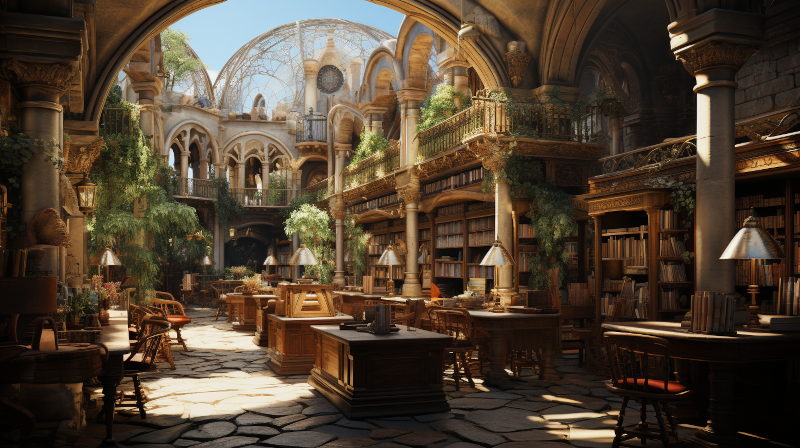
\includegraphics[width=500px]{./img/Ornasion-library-3.png}
\end{center}
This is the largest library in Naurrnen. It consists of a large citidel, with a castle and towers. It is primarily run by the Gran Imperio's Archivist Guild. The citidel consists of thousands of rooms deep under the surface of the city, and far into the chambers above the ground. Most of the transcriptions of the ancient books in Laurië Citime have been purchased and stored at this library.
\begin{enumerate}
\item The Archivist Guild: Guardians of Knowledge
\label{sec:org76779cd}
The Archivist Guild is the esteemed institution that serves as the backbone of Ornasion, the Citadel of Wisdom. Established in antiquity, this guild is a collective of the realm's most distinguished scholars, librarians, and documentarians whose primary mission is to preserve, catalog, and disseminate the vast reserves of knowledge stored within the city. With a focus that transcends mere bookkeeping, the Archivist Guild is committed to the promotion of intellectual curiosity and scholarly exchange across all disciplines.

Members of the guild undergo rigorous training in disciplines ranging from archival science to arcane arts, ensuring they possess the expertise required to maintain the complex web of knowledge housed in Ornasion. These archivists are more than just caretakers; they are mentors, guiding young scholars through the labyrinthine corridors of wisdom, and acting as mediators in intellectual debates and forums.

Once a year, the guild organizes the ``Conclave of Quills,'' an international symposium that invites scholars, historians, and researchers from far and wide to present their work, fostering an environment of academic collaboration and groundbreaking discoveries.

Additionally, the guild employs an elite force of mage-guards specially trained to safeguard the invaluable treasures of Ornasion. Utilizing a unique blend of martial skill and arcane knowledge, these mage-guards ensure the sanctity and security of one of Naurrnen's most invaluable resources.

The Archivist Guild is not just an organization; it's a living testament to Naurrnen’s commitment to the pursuit of knowledge. Through its ceaseless efforts, the guild ensures that the flame of intellectual inquiry continues to burn bright for future generations.
\end{enumerate}
\item Laurië Citime, Kingdon of Tanquende (Capital of Tanquende)
\label{sec:org5791b20}
\begin{center}
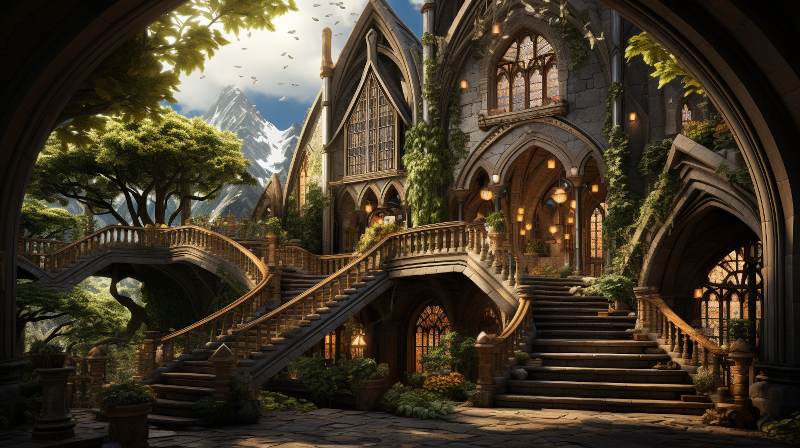
\includegraphics[width=500px]{./img/Laurie_Citime.png}
\end{center}
One of the oldest libraries in Naurrnen. Contains some of the oldest volumes known to civilization. There is also the largest Transcript guild within the city. The Transcript guild tries to make exact copies of the most ancient books within the library in an effort to preserve the books. They also make copies available to the printing presses, but these are considered inferior to the original books. Symbols, pictures, and sketches are of equal value to the printed word, and a book with just the printed word, contains only half the worth of the original. Lithography has been strictly prohibited within the Kingdom of Tanquende, so mass producing images in these arcane books are not currently legally possible. This also artificially inflates the value of the book copies made by the Transcript guilds.
\begin{enumerate}
\item The Transcript Guild: Preservers of Ancient Wisdom
\label{sec:org131df98}
Nestled in the heart of Laurië Citime, the Transcript Guild serves as a vanguard for the conservation and duplication of some of the most ancient and irreplaceable texts known to civilization. This esteemed institution is a sanctuary for scribes, artists, and scholars dedicated to the meticulous art of transcribing ancient works. While many guilds focus on the creation of new knowledge, the Transcript Guild specializes in the preservation of old wisdom, ensuring that it survives the ravages of time and circumstance.

Apprentices undergo years of stringent training, learning not only the art of exacting transcription but also mastering the antiquated languages and deciphering complex symbols and images. Among the Hallishim, it's a widely accepted notion that a text loses half its value when the rich tapestry of its original presentation is lost. Lithography may be forbidden within the Kingdom of Tanquende, but the hand-crafted volumes produced by the guild are considered invaluable, not just for their content but for their artisanal quality.

The guild enjoys a special partnership with the Archivist Guild of Ornasion, often exchanging texts and discoveries to further the preservation of knowledge across Naurrnen. The Transcript Guild also holds a sacred duty to analyze the encrypted riddles and codes found in works like ``The Ameara'' by Bayetti Falasha, seeking keys to unlock the deep secrets of the past.

In essence, the Transcript Guild is more than a guild; it is a living link between past and future, a bridge that allows the wisdom of ancient civilizations to enlighten the minds of generations yet unborn.
\end{enumerate}
\item Weylesbury, Gran Imperio (just a few miles south of Ponte Cidade).
\label{sec:org457bb40}
\begin{enumerate}
\item Home of University of Naethanor
\label{sec:org71ef657}
One of the most renowned Universities within Naurrnen. Named after Donnchadh and Elira (Elirandel) Naethanor. The university library hosts an intriquate marbel statue of Lady Naethanor.
\begin{center}
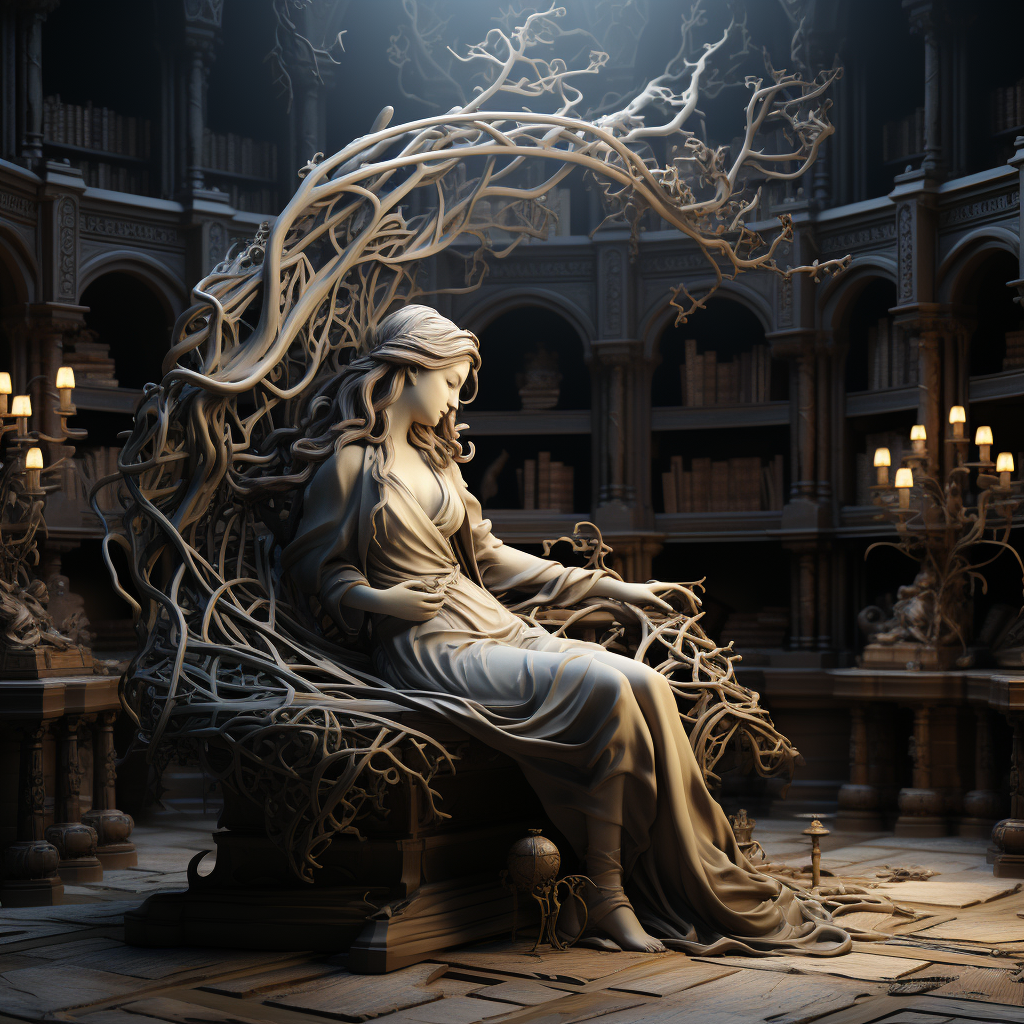
\includegraphics[width=500px]{./img/Elirandel.png}
\end{center}
\begin{enumerate}
\item Elira Naethanor
\label{sec:orge01bbbc}
Born to the prestigious royal line of Eärendelion, Elirandel was a prodigy among Elven scholars. She attended the esteemed Laurië Citime, where she studied a diverse range of subjects, from ancient lore to the arts of magic. Her future seemed predestined to be one of comfort and high standing within the Elven Empire of Átaremma.

Gifted in history, philosophy, and magical arts, she was poised for a future of influence and leadership within the empire. However, her life took a drastic turn when she befriended Cormac, an Adama slave serving at the institution. Intrigued by his curiosity about the Elven texts he couldn't read and drawn by his quiet yet profound intelligence, Elirandel made the daring decision to teach him how to read the Elven script.

This act was not merely taboo but considered treasonous, a rebellion against the very social fabric of Elven society. Teaching Cormac elevated him from a mere laborer to an intellectual peer, breaking longstanding racial and social barriers. As their friendship deepened into love and intellectual partnership, Elirandel began to question the ethics of the empire she was destined to serve.

Through secret meetings hidden amongst the labyrinthine library shelves, the pair discussed not just literature and history, but strategies for social reform. They shared dreams of an empire where Elven wisdom didn't oppress but uplifted all races. Cormac's intellectual prowess grew, and in turn, his political and strategic ideas began to shape Elirandel's understanding of justice and equality.

When it became increasingly clear that their intellectual pursuits and growing emotional bond could no longer be hidden, Elirandel had to make a life-altering choice. She chose love and justice over her secure, predetermined life. Faced with the threat of discovery, torture, and perhaps death, Elirandel and Cormac fled Laurië Citime to join an underground movement that aided slaves and political prisoners.

Elirandel's departure sent ripples through Elven society, marking her both as a traitor and a revolutionary icon. It was a price she was willing to pay. Together with Cormac, she would go on to challenge the might of Aerithia and lay the groundwork for what would become the Gran Imperio, forever changing the course of Naurrnen's history.
\item Cormac Naethanor
\label{sec:orgee03085}
Cormac was born into slavery, an Adama living under the oppressive rule of the Elven empire Aerithia. However, his life would diverge from the path of servitude most of his people walked when he was assigned to work at Laurië Citime, the foremost academic institution among the Elves. Although he started as a mere custodian of ancient tomes and scrolls, Cormac possessed an unquenchable thirst for knowledge and an innate intelligence that couldn't be ignored.

It was at Laurië Citime that Cormac met Elirandel Elenariel, a young Elven scholar of royal descent. Intrigued by his persistent questions and drawn to his untapped intellect, Elirandel took the risky step of teaching him how to read the Elven script. As he learned to decipher the intricate letters and understand complex philosophies, Cormac's worldview expanded, fueling his desire for social reform and justice for his people. He began to formulate innovative ideas that would later shape revolutionary strategies, greatly influencing Elirandel in return.

When their secret friendship blossomed into a forbidden romance and intellectual partnership, the risk of discovery grew ever more dangerous. Given Elirandel's high social status, their relationship was a volatile secret that could get them both killed. However, their intellectual and emotional connection couldn't be easily severed.

Faced with impending discovery, Cormac had to make an agonizing choice—stay and face almost certain execution, or flee with Elirandel to seek out the freedom fighters dedicated to the overthrow of Aerithia. Choosing the latter, he fled with the woman who had opened the world of letters to him, and whom he had enlightened in the ethics of justice and equality.

Together, they joined an underground movement that would eventually topple the mighty Elven empire and give rise to the Gran Imperio, a new realm founded on the principles they had dreamed of together. In doing so, Cormac would become not just a freed slave but a revolutionary leader, strategist, and one half of an iconic partnership that would change the course of history in Naurrnen.
\end{enumerate}
\end{enumerate}
\end{enumerate}

\subsection{Metals}
\label{sec:orgb8cee96}
\subsubsection{Saruleum}
\label{sec:orgac2298f}
\begin{enumerate}
\item From the ancient tongue (similar to Latin), meaning ``blue''.
\item Color is silver with streaks of blue light
\item Primary source of magicka
\item Primary source of energy
\item Is mined
\item Sometimes used as currency, but since it is generally softer than gold, it is not ideal for coinage.
\end{enumerate}

Saruleum is a soft metal and is an extremely inefficient energy source for magic, but an extremely efficient source of energy for mechanical contraptions. This means that cultures will view the resource as scarce, and better used for non-magical applications. Of course, the wizard guilds will want an unlimited supply of the resource so they can explore and learn more about magic.

\subsubsection{Baruleam}
\label{sec:org105d576}
A hard and heavy metal. Can be used as armor but is too heavy to make full suits of armor. Usually a plate of the metal will be used in conjunction with steel. It is most commonly used in constructs for production that need sturdy materials in order to function.

\subsubsection{Valmaur (Cruachlinn in the Adama tongue)}
\label{sec:org7660870}
Valmaur is a hard smooth-marble-like substance, but also durable. It has the same melting temprature of steel. But more maleable than steel. It is a poor conductor of heat, so it takes a long time to melt, but cools very quickly. It is an ideal substance in which to carve intricate statues. It's not as rare as Saruleum or Baruleam, but is still fairly uncommon.

\subsubsection{Steel}
\label{sec:org9525f79}
An alloy of carbon and iron. Treasured as a hard, yet portable metal, ideally used for weapons and armor.

\subsection{Trade}
\label{sec:orgf343190}
\subsubsection{Famous Trade Routes}
\label{sec:org2a0a49c}
\begin{enumerate}
\item Ponte Cidade
\label{sec:orgd8a2740}
Ponte Cidade or ``the bridge city'' is the capital of Gran Imperio or ``grand empire''. Since the fifth century of the third age, Ponte Cidade has been the trade capital of the known world. Goods from the farthest reaches flow to and forth from Ponte Cidade. Massive trade routes flowing from east to west and from north to south. Enriching many of the towns and cities along its trade routes. Gold, rare ores, and exotic food from the south, silks and fine garments from the east, smithing and magical items from the north. Shipping goods from the west. Religion and culture also spreads across the trade routes.
\begin{enumerate}
\item Indentured servitude
\label{sec:orgb4a1cdc}
Unlimited chartel slavery is strictly prohibited. Indentured servitude is used to help the poor and punish criminals. Indentured servitude comes with an expiration date, and if they are entitled to leave,  their masters must give them enough so they can self-sustain for at least 3 months after their departure. This keeps masters from trying to profit from the indentured servitude model.
\end{enumerate}
\end{enumerate}
\end{document}